

\documentclass[english]{article}\usepackage[]{graphicx}\usepackage[]{color}
%% maxwidth is the original width if it is less than linewidth
%% otherwise use linewidth (to make sure the graphics do not exceed the margin)
\makeatletter
\def\maxwidth{ %
  \ifdim\Gin@nat@width>\linewidth
    \linewidth
  \else
    \Gin@nat@width
  \fi
}
\makeatother

\definecolor{fgcolor}{rgb}{0.345, 0.345, 0.345}
\newcommand{\hlnum}[1]{\textcolor[rgb]{0.686,0.059,0.569}{#1}}%
\newcommand{\hlstr}[1]{\textcolor[rgb]{0.192,0.494,0.8}{#1}}%
\newcommand{\hlcom}[1]{\textcolor[rgb]{0.678,0.584,0.686}{\textit{#1}}}%
\newcommand{\hlopt}[1]{\textcolor[rgb]{0,0,0}{#1}}%
\newcommand{\hlstd}[1]{\textcolor[rgb]{0.345,0.345,0.345}{#1}}%
\newcommand{\hlkwa}[1]{\textcolor[rgb]{0.161,0.373,0.58}{\textbf{#1}}}%
\newcommand{\hlkwb}[1]{\textcolor[rgb]{0.69,0.353,0.396}{#1}}%
\newcommand{\hlkwc}[1]{\textcolor[rgb]{0.333,0.667,0.333}{#1}}%
\newcommand{\hlkwd}[1]{\textcolor[rgb]{0.737,0.353,0.396}{\textbf{#1}}}%
\let\hlipl\hlkwb

\usepackage{framed}
\makeatletter
\newenvironment{kframe}{%
 \def\at@end@of@kframe{}%
 \ifinner\ifhmode%
  \def\at@end@of@kframe{\end{minipage}}%
  \begin{minipage}{\columnwidth}%
 \fi\fi%
 \def\FrameCommand##1{\hskip\@totalleftmargin \hskip-\fboxsep
 \colorbox{shadecolor}{##1}\hskip-\fboxsep
     % There is no \\@totalrightmargin, so:
     \hskip-\linewidth \hskip-\@totalleftmargin \hskip\columnwidth}%
 \MakeFramed {\advance\hsize-\width
   \@totalleftmargin\z@ \linewidth\hsize
   \@setminipage}}%
 {\par\unskip\endMakeFramed%
 \at@end@of@kframe}
\makeatother

\definecolor{shadecolor}{rgb}{.97, .97, .97}
\definecolor{messagecolor}{rgb}{0, 0, 0}
\definecolor{warningcolor}{rgb}{1, 0, 1}
\definecolor{errorcolor}{rgb}{1, 0, 0}
\newenvironment{knitrout}{}{} % an empty environment to be redefined in TeX

\usepackage{alltt} % \documentclass[a4paper]{article}
\usepackage[T1]{fontenc}
\usepackage[latin9]{inputenc} % \usepackage[utf8]{inputenc}
\usepackage{geometry}
% \geometry{verbose,tmargin=2cm,bmargin=2cm,lmargin=3cm,rmargin=3cm}
\usepackage{amsthm, amsmath,amssymb} % ,amsfonts
\usepackage{setspace}
\usepackage{esint}
\usepackage[authoryear]{natbib}
\onehalfspacing

\makeatletter
\usepackage{authblk}
\usepackage[multiple]{footmisc}
\usepackage{pdflscape}
\usepackage{booktabs}

% \usepackage{jheppub}
%%\usepackage[round]{natbib}
\usepackage[colorlinks=true,urlcolor=blue]{hyperref}
\usepackage{graphicx}
\usepackage{pdflscape}
\usepackage{color}
\usepackage{float}

\definecolor{blue}{rgb}{.2,.2,.7}
\definecolor{red}{rgb}{.7,.2,.2}
\definecolor{green}{rgb}{0,.6,.3}
\definecolor{gray}{rgb}{0.45,0.45,0.45}
\newcommand{\btext}[1]{\textcolor{blue}{#1}}
\newcommand{\rtext}[1]{\textcolor{red}{#1}}
\newcommand{\gtext}[1]{\textcolor{green}{#1}}
\newcommand{\wtext}[1]{\textcolor{white}{#1}}
\newcommand{\old}[1]{\textcolor{gray}{#1}}
\definecolor{gray90}{RGB}{229,229,229}
\definecolor{gray77}{RGB}{196,196,196}
\definecolor{gray60}{RGB}{153,153,153}

\renewcommand{\thefootnote}{\alph{footnote}}
%%\newcommand{\acronym}[1]{\textsc{#1}}
%%\newcommand{\class}[1]{\mbox{\textsf{#1}}}
\newcommand{\code}[1]{\mbox{\texttt{#1}}}
\newcommand{\pkg}[1]{{\normalfont\fontseries{b}\selectfont #1}}
\newcommand{\proglang}[1]{\textsf{#1}}

\newcommand\XOR{\mathbin{\char`\^}}
\newcommand\independent{\protect\mathpalette{\protect\independenT}{\perp}}
\def\independenT#1#2{\mathrel{\rlap{$#1#2$}\mkern2mu{#1#2}}}

\theoremstyle{plain}
\newtheorem*{thm*}{\protect\theoremname}
\theoremstyle{plain}
\newtheorem*{lem*}{\protect\lemmaname}

\makeatother
\usepackage{babel}
\providecommand{\lemmaname}{Lemma}
\providecommand{\theoremname}{Theorem}


%\VignetteEngine{knitr::knitr}
%\VignetteIndexEntry{Introduction}


\IfFileExists{upquote.sty}{\usepackage{upquote}}{}
\begin{document}

% ------------------------------------------------------------
\section{Using R for Simulating Network-Dependent Observational Data}
% ------------------------------------------------------------

% % ------------------------------------------------------------
% \subsection{Defining the Data-Generating Distribution}
% % ------------------------------------------------------------

We start by defining the distribution of the observed network graph. In this example we choose the preferential attachment network model with power law node degree distribution, with the sampling function provided below.

\begin{knitrout}\footnotesize
\definecolor{shadecolor}{rgb}{0.969, 0.969, 0.969}\color{fgcolor}\begin{kframe}
\begin{alltt}
\hlkwd{require}\hlstd{(}\hlstr{"igraph"}\hlstd{)}
\hlkwd{require}\hlstd{(}\hlstr{"simcausal"}\hlstd{)}
\hlkwd{require}\hlstd{(}\hlstr{"ggraph"}\hlstd{)}
\hlstd{generate.igraph.prefattach} \hlkwb{<-} \hlkwa{function}\hlstd{(}\hlkwc{n}\hlstd{,} \hlkwc{power}\hlstd{,} \hlkwc{zero.appeal}\hlstd{,} \hlkwc{m}\hlstd{,} \hlkwc{...}\hlstd{) \{}
  \hlstd{g} \hlkwb{<-} \hlkwd{sample_pa}\hlstd{(n,} \hlkwc{power} \hlstd{= power,} \hlkwc{zero.appeal} \hlstd{= zero.appeal,} \hlkwc{m} \hlstd{= m)}
  \hlstd{g} \hlkwb{<-} \hlkwd{as.directed}\hlstd{(}\hlkwd{as.undirected}\hlstd{(g,} \hlkwc{mode} \hlstd{=} \hlstr{"collapse"}\hlstd{),} \hlkwc{mode} \hlstd{=} \hlstr{"mutual"}\hlstd{)}
  \hlstd{sparse_AdjMat} \hlkwb{<-} \hlstd{simcausal}\hlopt{::}\hlkwd{igraph.to.sparseAdjMat}\hlstd{(g)}
  \hlstd{NetInd_out} \hlkwb{<-} \hlstd{simcausal}\hlopt{::}\hlkwd{sparseAdjMat.to.NetInd}\hlstd{(sparse_AdjMat)}
  \hlkwd{return}\hlstd{(NetInd_out}\hlopt{$}\hlstd{NetInd_k)}
\hlstd{\}}
\end{alltt}
\end{kframe}
\end{knitrout}

The above network distribution is then added to a DAG object, which will define the observed data-generating distribution.

\begin{knitrout}\footnotesize
\definecolor{shadecolor}{rgb}{0.969, 0.969, 0.969}\color{fgcolor}\begin{kframe}
\begin{alltt}
\hlstd{D} \hlkwb{<-} \hlkwd{DAG.empty}\hlstd{()}
\hlstd{Net.prefattach} \hlkwb{<-} \hlkwd{network}\hlstd{(}\hlstr{"Net"}\hlstd{,} \hlkwc{netfun} \hlstd{=} \hlstr{"generate.igraph.prefattach"}\hlstd{,} \hlkwc{power} \hlstd{=} \hlnum{0.5}\hlstd{,} \hlkwc{zero.appeal} \hlstd{=} \hlnum{5}\hlstd{,} \hlkwc{m} \hlstd{=} \hlnum{5}\hlstd{)}
\end{alltt}
\end{kframe}
\end{knitrout}

Next, we define the distributions of the baseline covariates, as shown below. Note that we define the baseline indicator \texttt{HUB}, which indicates if a person has more or equal to 25 friends. We also define the baseline covariate \texttt{PA}, which indicates if a person is physically active at baseline and we define the network baseline summary \texttt{nF.PA}, which calculates the total number of friends of a person who are physically active.

\begin{knitrout}\footnotesize
\definecolor{shadecolor}{rgb}{0.969, 0.969, 0.969}\color{fgcolor}\begin{kframe}
\begin{alltt}
\hlstd{D} \hlkwb{<-} \hlstd{D} \hlopt{+} \hlstd{Net.prefattach} \hlopt{+}
  \hlkwd{node}\hlstd{(}\hlstr{"LatentW"}\hlstd{,} \hlkwc{distr} \hlstd{=} \hlstr{"rcat.b0"}\hlstd{,} \hlkwc{probs} \hlstd{=} \hlkwd{c}\hlstd{(}\hlnum{0.0494}\hlstd{,} \hlnum{0.1823}\hlstd{,} \hlnum{0.2806}\hlstd{,} \hlnum{0.2680}\hlstd{,}\hlnum{0.1651}\hlstd{,} \hlnum{0.0546}\hlstd{))} \hlopt{+}
  \hlkwd{node}\hlstd{(}\hlstr{"HUB"}\hlstd{,} \hlkwc{distr} \hlstd{=} \hlstr{"rconst"}\hlstd{,} \hlkwc{const} \hlstd{=} \hlkwd{ifelse}\hlstd{(nF} \hlopt{>=} \hlnum{25}\hlstd{,} \hlnum{1}\hlstd{,} \hlnum{0}\hlstd{))} \hlopt{+}
  \hlkwd{node}\hlstd{(}\hlstr{"W1"}\hlstd{,} \hlkwc{distr} \hlstd{=} \hlstr{"rcat.b1"}\hlstd{,} \hlkwc{probs} \hlstd{=} \hlkwd{c}\hlstd{(}\hlnum{0.0494}\hlstd{,} \hlnum{0.1823}\hlstd{,} \hlnum{0.2806}\hlstd{,} \hlnum{0.2680}\hlstd{,}\hlnum{0.1651}\hlstd{,} \hlnum{0.0546}\hlstd{))} \hlopt{+}
  \hlkwd{node}\hlstd{(}\hlstr{"W2"}\hlstd{,} \hlkwc{distr} \hlstd{=} \hlstr{"rbern"}\hlstd{,} \hlkwc{prob} \hlstd{=} \hlkwd{plogis}\hlstd{(}\hlopt{-}\hlnum{0.2}\hlstd{))} \hlopt{+}
  \hlkwd{node}\hlstd{(}\hlstr{"WNoise"}\hlstd{,} \hlkwc{distr} \hlstd{=} \hlstr{"rbern"}\hlstd{,} \hlkwc{prob} \hlstd{=} \hlkwd{plogis}\hlstd{(}\hlopt{-}\hlnum{0.4}\hlstd{))} \hlopt{+}
  \hlkwd{node}\hlstd{(}\hlstr{"corrW.F1"}\hlstd{,} \hlkwc{distr} \hlstd{=} \hlstr{"rbern"}\hlstd{,} \hlkwc{prob} \hlstd{=} \hlkwd{plogis}\hlstd{(}\hlopt{-}\hlnum{8} \hlopt{+} \hlnum{2}\hlopt{*}\hlstd{LatentW} \hlopt{+} \hlnum{2}\hlopt{*}\hlstd{LatentW))} \hlopt{+}
  \hlkwd{node}\hlstd{(}\hlstr{"corrW.F2"}\hlstd{,} \hlkwc{distr} \hlstd{=} \hlstr{"rbern"}\hlstd{,} \hlkwc{prob} \hlstd{=} \hlkwd{plogis}\hlstd{(}\hlopt{-}\hlnum{6} \hlopt{+} \hlnum{1.5}\hlopt{*}\hlstd{LatentW} \hlopt{+} \hlnum{1.5}\hlopt{*}\hlstd{LatentW))} \hlopt{+}
  \hlkwd{node}\hlstd{(}\hlstr{"corrW.F3"}\hlstd{,} \hlkwc{distr} \hlstd{=} \hlstr{"rbern"}\hlstd{,} \hlkwc{prob} \hlstd{=} \hlkwd{plogis}\hlstd{(}\hlopt{-}\hlnum{6} \hlopt{+} \hlnum{1.5}\hlopt{*}\hlstd{LatentW} \hlopt{+} \hlnum{1.5}\hlopt{*}\hlstd{LatentW))} \hlopt{+}
  \hlkwd{node}\hlstd{(}\hlstr{"corrW.F4"}\hlstd{,} \hlkwc{distr} \hlstd{=} \hlstr{"rbern"}\hlstd{,} \hlkwc{prob} \hlstd{=} \hlkwd{plogis}\hlstd{(}\hlopt{-}\hlnum{4} \hlopt{+} \hlstd{LatentW} \hlopt{+} \hlstd{LatentW))} \hlopt{+}
  \hlkwd{node}\hlstd{(}\hlstr{"corrW.F5"}\hlstd{,} \hlkwc{distr} \hlstd{=} \hlstr{"rbern"}\hlstd{,} \hlkwc{prob} \hlstd{=} \hlkwd{plogis}\hlstd{(}\hlopt{-}\hlnum{4} \hlopt{+} \hlstd{LatentW} \hlopt{+} \hlstd{LatentW))} \hlopt{+}
\hlcom{# Status of being physically active at baseline:}
  \hlkwd{node}\hlstd{(}\hlstr{"PA"}\hlstd{,} \hlkwc{distr} \hlstd{=} \hlstr{"rbern"}\hlstd{,} \hlkwc{prob} \hlstd{= W2}\hlopt{*}\hlnum{0.05} \hlopt{+} \hlstd{(}\hlnum{1}\hlopt{-}\hlstd{W2)}\hlopt{*}\hlnum{0.15}\hlstd{)} \hlopt{+}
\hlcom{# Total number of physically active friends:}
  \hlkwd{node}\hlstd{(}\hlstr{"nF.PA"}\hlstd{,} \hlkwc{distr} \hlstd{=} \hlstr{"rconst"}\hlstd{,} \hlkwc{const} \hlstd{=} \hlkwd{sum}\hlstd{(PA[[}\hlnum{1}\hlopt{:}\hlstd{Kmax]]),} \hlkwc{replaceNAw0} \hlstd{=} \hlnum{TRUE}\hlstd{)}
\end{alltt}
\end{kframe}
\end{knitrout}

As a next step we randomly assign the binary exposure, \texttt{A}, to 25\% of the population. This exposure corresponds with an informational campaign about the benefits of physical exercise and is intended to promote and sustain attendance of the local gym by community members.

\begin{knitrout}\footnotesize
\definecolor{shadecolor}{rgb}{0.969, 0.969, 0.969}\color{fgcolor}\begin{kframe}
\begin{alltt}
\hlstd{D} \hlkwb{<-} \hlstd{D} \hlopt{+} \hlkwd{node}\hlstd{(}\hlstr{"A"}\hlstd{,} \hlkwc{distr} \hlstd{=} \hlstr{"rbern"}\hlstd{,} \hlkwc{prob} \hlstd{=} \hlnum{0.25}\hlstd{)}
\end{alltt}
\end{kframe}
\end{knitrout}

Next, we define some network summary measure, \texttt{sum.net.A3}, as shown below, which depends on the exposures of individuals' friends, as well as their friends' baseline covariate values.


\begin{knitrout}\footnotesize
\definecolor{shadecolor}{rgb}{0.969, 0.969, 0.969}\color{fgcolor}\begin{kframe}
\begin{alltt}
\hlstd{D} \hlkwb{<-} \hlstd{D} \hlopt{+} \hlkwd{node}\hlstd{(}\hlstr{"sum.net.A"}\hlstd{,} \hlkwc{distr} \hlstd{=} \hlstr{"rconst"}\hlstd{,}
  \hlkwc{const} \hlstd{= (}\hlkwd{sum}\hlstd{(A[[}\hlnum{1}\hlopt{:}\hlstd{Kmax]])}\hlopt{*}\hlstd{(HUB}\hlopt{==}\hlnum{0}\hlstd{)} \hlopt{+} \hlkwd{sum}\hlstd{((W1[[}\hlnum{1}\hlopt{:}\hlstd{Kmax]]} \hlopt{>} \hlnum{4}\hlstd{)}\hlopt{*}\hlstd{A[[}\hlnum{1}\hlopt{:}\hlstd{Kmax]])}\hlopt{*}\hlstd{(HUB}\hlopt{==}\hlnum{1}\hlstd{)),}
  \hlkwc{replaceNAw0} \hlstd{=} \hlnum{TRUE}\hlstd{)}
\end{alltt}
\end{kframe}
\end{knitrout}

We define the binary outcome \texttt{Y} below, which is defined as an indicator of sustaining a membership in a local gym for the duration of 6 months following the intervention \texttt{A}. Note that we assumed that each \texttt{Y} depends on the individual exposure and baseline covariates. It also depends on the network summary \texttt{sum.net.A3} defined above, as well as \texttt{nF.PA}, which represents the total number of friends of the individual who were physically active \texttt{PA=1} at baseline.

\begin{knitrout}\footnotesize
\definecolor{shadecolor}{rgb}{0.969, 0.969, 0.969}\color{fgcolor}\begin{kframe}
\begin{alltt}
\hlstd{D} \hlkwb{<-} \hlstd{D} \hlopt{+}
  \hlkwd{node}\hlstd{(}\hlstr{"Y"}\hlstd{,} \hlkwc{distr} \hlstd{=} \hlstr{"rbern"}\hlstd{,} \hlkwc{prob} \hlstd{=} \hlkwd{plogis}\hlstd{(}\hlkwd{ifelse}\hlstd{(PA} \hlopt{==} \hlnum{1}\hlstd{,}
    \hlopt{+}\hlnum{5} \hlopt{-} \hlnum{15}\hlopt{*}\hlstd{(nF.PA} \hlopt{<} \hlnum{1}\hlstd{),}
    \hlopt{-}\hlnum{8.0} \hlopt{+} \hlnum{0.25}\hlopt{*}\hlstd{A)} \hlopt{+}
    \hlopt{+}\hlnum{0.5}\hlopt{*}\hlstd{sum.net.A} \hlopt{+} \hlnum{0.25}\hlopt{*}\hlstd{nF.PA}\hlopt{*}\hlstd{sum.net.A} \hlopt{+} \hlnum{0.5}\hlopt{*}\hlstd{nF.PA} \hlopt{+}
    \hlopt{+}\hlnum{0.5}\hlopt{*}\hlstd{(W1}\hlopt{-}\hlnum{1}\hlstd{)} \hlopt{-} \hlnum{0.58}\hlopt{*}\hlstd{W2} \hlopt{+}
    \hlopt{-}\hlnum{0.5}\hlopt{*}\hlstd{(}\hlnum{3.477}\hlopt{-}\hlnum{1}\hlstd{)} \hlopt{+} \hlnum{0.58}\hlopt{*}\hlnum{0.4496} \hlopt{+}
    \hlopt{+}\hlnum{4}\hlopt{*}\hlstd{corrW.F1} \hlopt{-}\hlnum{2}\hlopt{*}\hlstd{corrW.F2} \hlopt{-}\hlnum{2}\hlopt{*}\hlstd{corrW.F3} \hlopt{+}\hlnum{2}\hlopt{*}\hlstd{corrW.F4} \hlopt{-}\hlnum{2}\hlopt{*}\hlstd{corrW.F5} \hlopt{+}
    \hlopt{-}\hlnum{4}\hlopt{*}\hlnum{0.6841}   \hlopt{+}\hlnum{2}\hlopt{*}\hlnum{0.6727}   \hlopt{+}\hlnum{2}\hlopt{*}\hlnum{0.6724}   \hlopt{-}\hlnum{2}\hlopt{*}\hlnum{0.6513}   \hlopt{+}\hlnum{2}\hlopt{*}\hlnum{0.6538}\hlstd{),}
    \hlkwc{replaceNAw0} \hlstd{=} \hlnum{TRUE}\hlstd{)}
\end{alltt}
\end{kframe}
\end{knitrout}

Finally, we define the data-generating distribution based on the preferential attachment network model, as shown below.

\begin{knitrout}\footnotesize
\definecolor{shadecolor}{rgb}{0.969, 0.969, 0.969}\color{fgcolor}\begin{kframe}
\begin{alltt}
\hlstd{D.prefattach} \hlkwb{<-} \hlkwd{set.DAG}\hlstd{(D,} \hlkwc{latent.v} \hlstd{=} \hlkwd{c}\hlstd{(}\hlstr{"LatentW"}\hlstd{),} \hlkwc{n.test} \hlstd{=} \hlnum{200}\hlstd{)}
\end{alltt}
\end{kframe}
\end{knitrout}


We now call function \code{sim} to simulate a single network of 5,000 individuals using the above defined data-generating distribution, as shown below. We also look at the distribution of node connectivity in Figure \textbf{X.X} and we plot this network for a small sample of 50 observations in Figure \textbf{X.X}

\begin{knitrout}\footnotesize
\definecolor{shadecolor}{rgb}{0.969, 0.969, 0.969}\color{fgcolor}\begin{kframe}
\begin{alltt}
\hlstd{datO_5K} \hlkwb{<-} \hlkwd{sim}\hlstd{(D.prefattach,} \hlkwc{n} \hlstd{=} \hlnum{5000}\hlstd{)}
\end{alltt}
\end{kframe}
\end{knitrout}

\begin{knitrout}\footnotesize
\definecolor{shadecolor}{rgb}{0.969, 0.969, 0.969}\color{fgcolor}\begin{figure}[ht]

{\centering 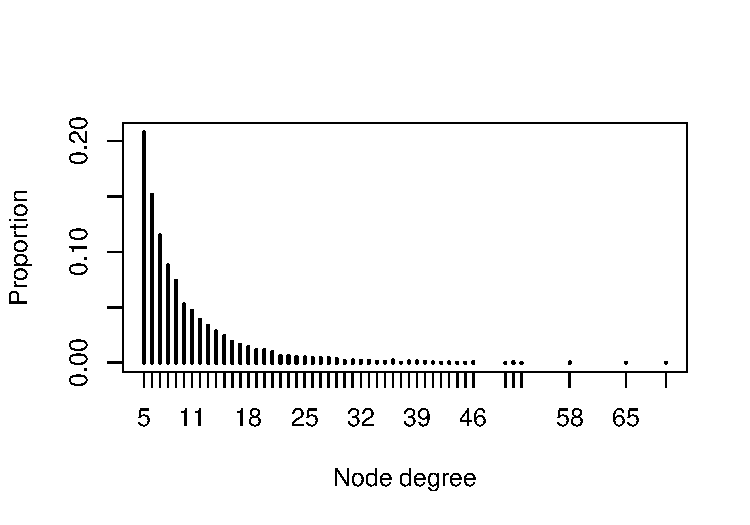
\includegraphics[width=\maxwidth]{TablesFigs/knitR-unnamed-chunk-10-1} 

}

\caption[Degree distribution for a preferential attachment network with 5,000 observations]{Degree distribution for a preferential attachment network with 5,000 observations.}\label{fig:unnamed-chunk-10}
\end{figure}


\end{knitrout}

\begin{knitrout}\footnotesize
\definecolor{shadecolor}{rgb}{0.969, 0.969, 0.969}\color{fgcolor}\begin{figure}[ht]

{\centering 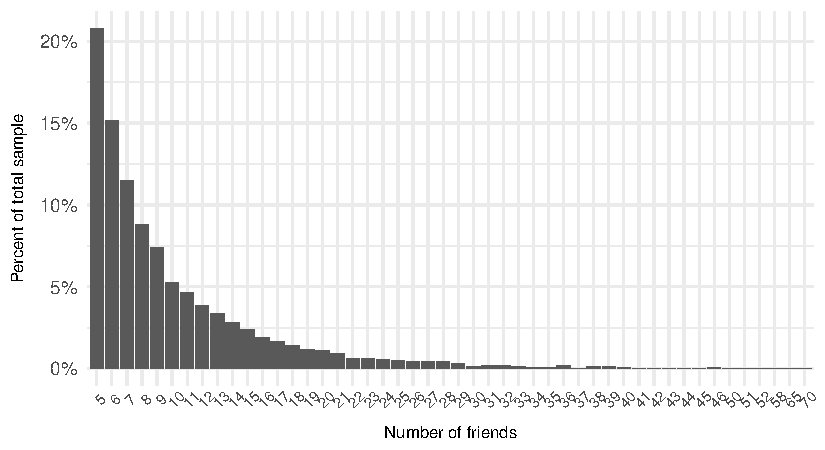
\includegraphics[width=\maxwidth]{TablesFigs/knitR-unnamed-chunk-11-1} 

}

\caption[Degree distribution for a preferential attachment network with 5,000 observations]{Degree distribution for a preferential attachment network with 5,000 observations.}\label{fig:unnamed-chunk-11}
\end{figure}


\end{knitrout}


\begin{knitrout}\footnotesize
\definecolor{shadecolor}{rgb}{0.969, 0.969, 0.969}\color{fgcolor}\begin{figure}[ht]

{\centering 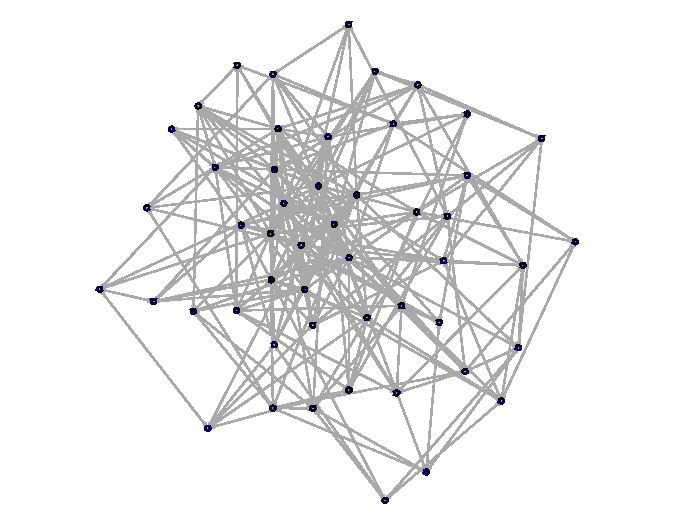
\includegraphics[width=\maxwidth]{TablesFigs/knitR-unnamed-chunk-12-1} 

}

\caption{Example of a preferential attachment network for 50 observations.\label{fig:netExamplePA}}\label{fig:unnamed-chunk-12}
\end{figure}


\end{knitrout}

\begin{knitrout}\footnotesize
\definecolor{shadecolor}{rgb}{0.969, 0.969, 0.969}\color{fgcolor}\begin{kframe}


{\ttfamily\noindent\color{warningcolor}{\#\# Warning: package 'bindrcpp' was built under R version 3.3.2}}\end{kframe}\begin{figure}[ht]

{\centering 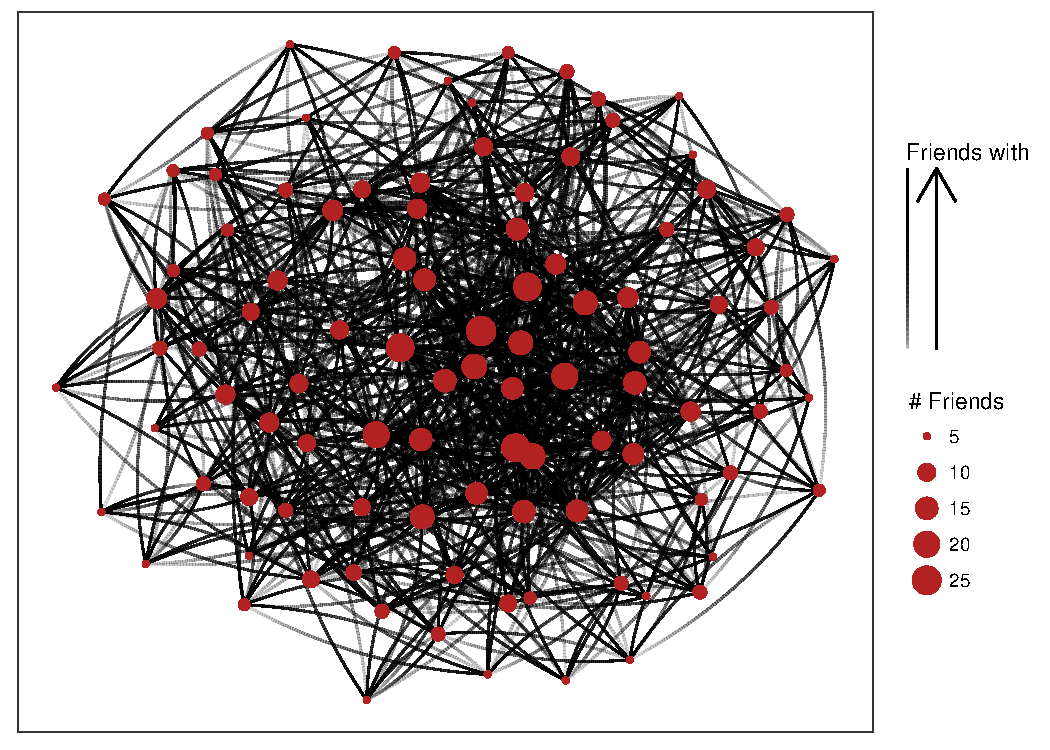
\includegraphics[width=\maxwidth]{TablesFigs/knitR-unnamed-chunk-13-1} 

}

\caption{Alternative representation of the same preferential attachment network for 100 observations.\label{fig:netExamplePA2}}\label{fig:unnamed-chunk-13}
\end{figure}


\end{knitrout}

\begin{knitrout}\footnotesize
\definecolor{shadecolor}{rgb}{0.969, 0.969, 0.969}\color{fgcolor}\begin{figure}[ht]

{\centering 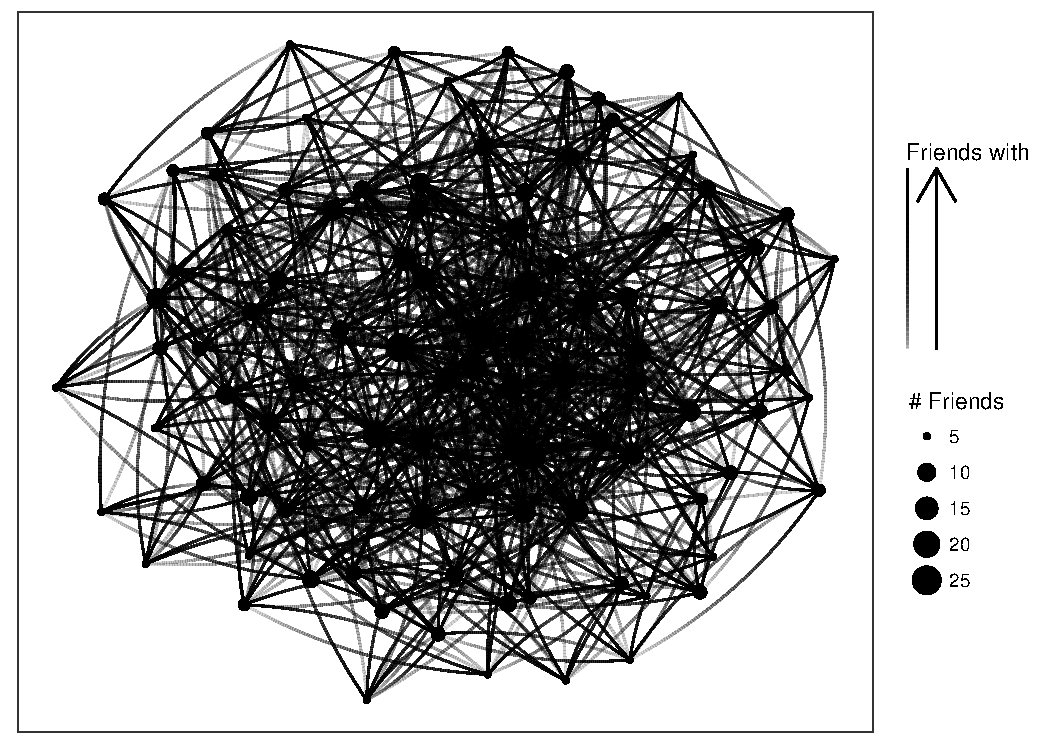
\includegraphics[width=\maxwidth]{TablesFigs/knitR-unnamed-chunk-14-1} 

}

\caption{Alternative representation of the same preferential attachment network for 100 observations.\label{fig:netExamplePA2.bw}}\label{fig:unnamed-chunk-14}
\end{figure}


\end{knitrout}

% ------------------------------------------------------------
\subsection{Evaluating Target Causal Quantities from Simulated Counterfactual Data}
% ------------------------------------------------------------

Next we define several stochastic and dynamic interventions on the exposure \texttt{A}, as well as the total number of physically active friends \texttt{nF.PA}. We also calculate the corresponding causal effects of these interventions, using the preferential attachment network model. Note that one can easily evaluate the true values of the above causal parameters by simulating intervention-specific counterfactual data and then evaluating the estimated mean of the counterfactual outcomes, as shown in all of the following examples.

Mean causal outcome under 35\% random coverage:

\begin{knitrout}\footnotesize
\definecolor{shadecolor}{rgb}{0.969, 0.969, 0.969}\color{fgcolor}\begin{kframe}
\begin{alltt}
\hlstd{D.prefattach} \hlkwb{<-} \hlstd{D.prefattach} \hlopt{+}
  \hlkwd{action}\hlstd{(}\hlstr{"gstar"}\hlstd{,} \hlkwc{nodes} \hlstd{=} \hlkwd{node}\hlstd{(}\hlstr{"A"}\hlstd{,} \hlkwc{distr} \hlstd{=} \hlstr{"rbern"}\hlstd{,} \hlkwc{prob} \hlstd{= aset),} \hlkwc{aset} \hlstd{=} \hlnum{0.35}\hlstd{)}
\hlstd{datFull} \hlkwb{<-} \hlkwd{sim}\hlstd{(D.prefattach,} \hlkwc{actions}\hlstd{=}\hlstr{"gstar"}\hlstd{,} \hlkwc{n} \hlstd{=} \hlnum{50000}\hlstd{,} \hlkwc{rndseed} \hlstd{=} \hlnum{54321}\hlstd{)}
\hlkwd{print}\hlstd{(psi0_a0.4} \hlkwb{<-} \hlkwd{mean}\hlstd{(datFull[[}\hlstr{"gstar"}\hlstd{]]}\hlopt{$}\hlstd{Y))}
\end{alltt}
\begin{verbatim}
## [1] 0.15186
\end{verbatim}
\end{kframe}
\end{knitrout}

Dynamic intervention that covers only around 10\% of the population by intervening (stochastically) only on the most connected individuals:

\begin{knitrout}\footnotesize
\definecolor{shadecolor}{rgb}{0.969, 0.969, 0.969}\color{fgcolor}\begin{kframe}
\begin{alltt}
\hlstd{D.prefattach} \hlkwb{<-} \hlstd{D.prefattach} \hlopt{+}
\hlkwd{action}\hlstd{(}\hlstr{"gHubs"}\hlstd{,}
  \hlkwc{nodes} \hlstd{=} \hlkwd{c}\hlstd{(}\hlkwd{node}\hlstd{(}\hlstr{"A"}\hlstd{,} \hlkwc{distr} \hlstd{=} \hlstr{"rbern"}\hlstd{,} \hlkwc{prob} \hlstd{=} \hlkwd{ifelse}\hlstd{(nF} \hlopt{>=} \hlnum{20}\hlstd{,} \hlnum{0.9}\hlstd{,} \hlkwd{ifelse}\hlstd{(nF} \hlopt{>=} \hlnum{15}\hlstd{,} \hlnum{0.40}\hlstd{,} \hlnum{0}\hlstd{)))))}
\hlstd{datFull} \hlkwb{<-} \hlkwd{sim}\hlstd{(D.prefattach,} \hlkwc{actions}\hlstd{=}\hlstr{"gHubs"}\hlstd{,} \hlkwc{n} \hlstd{=} \hlnum{50000}\hlstd{,} \hlkwc{rndseed} \hlstd{=} \hlnum{54321}\hlstd{)}
\hlkwd{print}\hlstd{(psi0_g.dynamic} \hlkwb{<-} \hlkwd{mean}\hlstd{(datFull[[}\hlstr{"gHubs"}\hlstd{]]}\hlopt{$}\hlstd{Y))}
\end{alltt}
\begin{verbatim}
## [1] 0.1204
\end{verbatim}
\end{kframe}
\end{knitrout}

Network intervention that increases the number of physically active friends by 1:

\begin{knitrout}\footnotesize
\definecolor{shadecolor}{rgb}{0.969, 0.969, 0.969}\color{fgcolor}\begin{kframe}
\begin{alltt}
\hlstd{D.prefattach} \hlkwb{<-} \hlstd{D.prefattach} \hlopt{+}
  \hlkwd{action}\hlstd{(}\hlstr{"plus.nF.PA"}\hlstd{,}
    \hlkwc{nodes} \hlstd{=} \hlkwd{node}\hlstd{(}\hlstr{"nF.PA"}\hlstd{,} \hlkwc{distr} \hlstd{=} \hlstr{"rconst"}\hlstd{,}
      \hlkwc{const} \hlstd{=} \hlkwd{ifelse}\hlstd{(nF} \hlopt{<=} \hlnum{15}\hlstd{,} \hlkwd{sum}\hlstd{(PA[[}\hlnum{1}\hlopt{:}\hlstd{Kmax]])} \hlopt{+} \hlnum{1}\hlstd{,}
                     \hlkwd{sum}\hlstd{(PA[[}\hlnum{1}\hlopt{:}\hlstd{Kmax]])),}
      \hlkwc{replaceNAw0} \hlstd{=} \hlnum{TRUE}\hlstd{))}
\hlstd{datFull} \hlkwb{<-} \hlkwd{sim}\hlstd{(D.prefattach,} \hlkwc{actions}\hlstd{=}\hlstr{"plus.nF.PA"}\hlstd{,} \hlkwc{n} \hlstd{=} \hlnum{50000}\hlstd{,} \hlkwc{rndseed} \hlstd{=} \hlnum{54321}\hlstd{)}
\hlkwd{print}\hlstd{(psi0_plusnF.PA} \hlkwb{<-} \hlkwd{mean}\hlstd{(datFull[[}\hlstr{"plus.nF.PA"}\hlstd{]]}\hlopt{$}\hlstd{Y))}
\end{alltt}
\begin{verbatim}
## [1] 0.17822
\end{verbatim}
\end{kframe}
\end{knitrout}

% ------------------------------------------------------------
\section{Estimation of causal effects for network dependent data}
% ------------------------------------------------------------

Having defined the simulated network data, as well as the true value of the target causal quantity (the gold standard), we switch to the topic of using R for estimating such causal parameters.


\paragraph{Network-based summary measures}
Example below.

\begin{knitrout}\footnotesize
\definecolor{shadecolor}{rgb}{0.969, 0.969, 0.969}\color{fgcolor}\begin{kframe}
\begin{alltt}
\hlkwd{require}\hlstd{(}\hlstr{"tmlenet"}\hlstd{)}

\hlstd{sW} \hlkwb{<-} \hlkwd{def_sW}\hlstd{(W1, W2, W3)} \hlopt{+}
  \hlkwd{def_sW}\hlstd{(}\hlkwc{W1.W2} \hlstd{= W1} \hlopt{*} \hlstd{W2)} \hlopt{+}
  \hlkwd{def_sW}\hlstd{(}\hlkwc{mW1.W2} \hlstd{= (}\hlnum{1} \hlopt{-} \hlstd{W1)} \hlopt{*} \hlstd{(}\hlnum{1} \hlopt{-} \hlstd{W2))} \hlopt{+}
  \hlkwd{def_sW}\hlstd{(}\hlkwc{W1.W3} \hlstd{= W1} \hlopt{*} \hlstd{W3)} \hlopt{+}
  \hlkwd{def_sW}\hlstd{(}\hlkwc{mW1.W3} \hlstd{= (}\hlnum{1} \hlopt{-} \hlstd{W1)} \hlopt{*} \hlstd{(}\hlnum{1} \hlopt{-} \hlstd{W3))} \hlopt{+}
  \hlkwd{def_sW}\hlstd{(}\hlkwc{W2.W3} \hlstd{= W2} \hlopt{*} \hlstd{W3)} \hlopt{+}
  \hlkwd{def_sW}\hlstd{(}\hlkwc{mW2.W3} \hlstd{= (}\hlnum{1} \hlopt{-} \hlstd{W2)} \hlopt{*} \hlstd{(}\hlnum{1} \hlopt{-} \hlstd{W3))} \hlopt{+}
  \hlkwd{def_sW}\hlstd{(}\hlkwc{net.mean.W1} \hlstd{=} \hlkwd{ifelse}\hlstd{(nF} \hlopt{>} \hlnum{0}\hlstd{,} \hlkwd{rowSums}\hlstd{(W1[[}\hlnum{1}\hlopt{:}\hlstd{Kmax]])}\hlopt{/}\hlstd{nF,} \hlnum{0}\hlstd{),} \hlkwc{replaceNAw0} \hlstd{=} \hlnum{TRUE}\hlstd{)}

\hlstd{sA} \hlkwb{<-} \hlkwd{def_sA}\hlstd{(sA,} \hlkwc{net.mean.sA} \hlstd{=} \hlkwd{sum}\hlstd{(sA[[}\hlnum{1}\hlopt{:}\hlstd{Kmax]])}\hlopt{/}\hlstd{nF,} \hlkwc{replaceNAw0} \hlstd{=} \hlnum{TRUE}\hlstd{)}
\end{alltt}
\end{kframe}
\end{knitrout}

Using \proglang{R} to define the summary measures with the \pkg{tmlenet} package.

\begin{knitrout}\footnotesize
\definecolor{shadecolor}{rgb}{0.969, 0.969, 0.969}\color{fgcolor}\begin{kframe}
\begin{alltt}
\hlstd{sW} \hlkwb{<-}  \hlkwd{def_sW}\hlstd{(W1, W2, WNoise, corrW.F1, corrW.F2, corrW.F3, corrW.F4, corrW.F5,}
  \hlkwc{HUB} \hlstd{=} \hlkwd{ifelse}\hlstd{(nF} \hlopt{>=} \hlnum{25}\hlstd{,} \hlnum{1}\hlstd{,} \hlnum{0}\hlstd{))}
\end{alltt}


{\ttfamily\noindent\itshape\color{messagecolor}{\#\# Some summary measures were not named, automatic column name(s) will be generated during evaluation}}\begin{alltt}
\hlstd{sA} \hlkwb{<-}  \hlkwd{def_sA}\hlstd{(A,} \hlkwc{nF.PA} \hlstd{=} \hlkwd{sum}\hlstd{(PA[[}\hlnum{1}\hlopt{:}\hlstd{Kmax]]),} \hlkwc{replaceNAw0} \hlstd{=} \hlnum{TRUE}\hlstd{)} \hlopt{+}
 \hlkwd{def_sA}\hlstd{(}\hlkwc{A.PAeq0} \hlstd{= A} \hlopt{*} \hlstd{(PA} \hlopt{==} \hlnum{0}\hlstd{))} \hlopt{+}
 \hlkwd{def_sA}\hlstd{(}\hlkwc{nFPAeq0.PAeq1} \hlstd{= (nF.PA} \hlopt{<} \hlnum{1}\hlstd{)} \hlopt{*} \hlstd{(PA} \hlopt{==} \hlnum{1}\hlstd{))} \hlopt{+}
 \hlkwd{def_sA}\hlstd{(}\hlkwc{sum.net.A} \hlstd{= (}\hlkwd{sum}\hlstd{(A[[}\hlnum{1}\hlopt{:}\hlstd{Kmax]])}\hlopt{*}\hlstd{(HUB}\hlopt{==}\hlnum{0}\hlstd{)} \hlopt{+} \hlkwd{sum}\hlstd{((W1[[}\hlnum{1}\hlopt{:}\hlstd{Kmax]]} \hlopt{>} \hlnum{4}\hlstd{)}\hlopt{*}\hlstd{A[[}\hlnum{1}\hlopt{:}\hlstd{Kmax]])}\hlopt{*}\hlstd{(HUB}\hlopt{==}\hlnum{1}\hlstd{)),}
        \hlkwc{sum.net.A.sum.netPA} \hlstd{= sum.net.A}\hlopt{*}\hlstd{nF.PA,}
        \hlkwc{replaceNAw0} \hlstd{=} \hlnum{TRUE}\hlstd{)}
\end{alltt}


{\ttfamily\noindent\itshape\color{messagecolor}{\#\# Some summary measures were not named, automatic column name(s) will be generated during evaluation}}\end{kframe}
\end{knitrout}

\paragraph{Regression models}

Examples of model specifications for the outcome and the \textit{effective exposure} models.

\begin{knitrout}\footnotesize
\definecolor{shadecolor}{rgb}{0.969, 0.969, 0.969}\color{fgcolor}\begin{kframe}
\begin{alltt}
\hlstd{Qforms} \hlkwb{<-} \hlstr{"Y ~ nF.PA + A.PAeq0 + nFPAeq0.PAeq1 + sum.net.A + sum.net.A.sum.netPA + PA + W1 + W2 + corrW.F1 + corrW.F2 + corrW.F3 + corrW.F4 + corrW.F5"}
\hlstd{hform} \hlkwb{<-} \hlstr{"A + sum.net.A ~ HUB + PA + nF.PA + nFPAeq0.PAeq1"}
\end{alltt}
\end{kframe}
\end{knitrout}

\paragraph{Interventions}

Examples of interventions on summary measures.

\begin{enumerate}
\item{All intervention nodes must be named and must match some previously defined summary measure/node name (been previously defined in  \texttt{def\_sA}).}
\item{The interention nodes/summaries will replace the existing ones.}
\item{The summaries that were part of  \texttt{def\_sA} and were not re-defined in  \texttt{def\_sA.gstar} will be  still re-evaluated on the data generated under  \texttt{def\_sA.gstar.}}
\item{Each intervention nodes/summary can reference the value of its own previously defined node, evaluated under observed data. For example, if we had an observed binary exposure data column A (registered with \texttt{def\_sA(A)}), the intervention that reverses the value of A from 0 to 1 and from 1 to 0 could be simply defined as \texttt{def\_sA.gstar(A = 1 - A)}.}
\item{All of the observed exposure summaries defined in obs.sW.sA are evaluated in EXACTLY the same order as they were defined. Hence all the intervention summaries preserve exactly the same order of evaluation as in \texttt{obs.sW.sA}.}
\end{enumerate}

\begin{knitrout}\footnotesize
\definecolor{shadecolor}{rgb}{0.969, 0.969, 0.969}\color{fgcolor}\begin{kframe}
\begin{alltt}
\hlcom{# Example 1A: Increase the total number of phys-active friends by 1.}
\hlstd{sA_star1a} \hlkwb{<-} \hlkwd{def_new_sA}\hlstd{(}\hlkwc{nF.PA} \hlstd{= (nF} \hlopt{<=} \hlnum{10}\hlstd{)}\hlopt{*}\hlstd{(}\hlkwd{sum}\hlstd{(PA[[}\hlnum{1}\hlopt{:}\hlstd{Kmax]])}\hlopt{+}\hlnum{1}\hlstd{)} \hlopt{+} \hlstd{(nF} \hlopt{>} \hlnum{10}\hlstd{)}\hlopt{*}\hlkwd{sum}\hlstd{(PA[[}\hlnum{1}\hlopt{:}\hlstd{Kmax]]),} \hlkwc{replaceNAw0} \hlstd{=} \hlnum{TRUE}\hlstd{)}
\hlcom{# # Example 1B: Alternative way of defining exactly the same intervention (will over-ride the existing summary nF.PA defined under sA)}
\hlstd{sA_star1b} \hlkwb{<-} \hlkwd{def_new_sA}\hlstd{(}\hlkwc{nF.PA} \hlstd{= (nF} \hlopt{<=} \hlnum{10}\hlstd{)}\hlopt{*}\hlstd{(nF.PA}\hlopt{+}\hlnum{1}\hlstd{)} \hlopt{+} \hlstd{(nF} \hlopt{>} \hlnum{10}\hlstd{)}\hlopt{*}\hlstd{nF.PA)}
\hlcom{# Example 2: Sample A as a stochastic intervention:}
\hlstd{sA_star2} \hlkwb{<-}  \hlkwd{def_new_sA}\hlstd{(}\hlkwc{A} \hlstd{=} \hlkwd{rbinom}\hlstd{(}\hlkwc{n} \hlstd{=} \hlkwd{length}\hlstd{(A),} \hlkwc{size} \hlstd{=} \hlnum{1}\hlstd{,} \hlkwc{prob} \hlstd{=} \hlnum{0.10}\hlstd{))}
\hlcom{# Example 3A: Sample A as a stochastic intervention and don't intervene on the summaries of the HUBS:}
\hlstd{sA_star3a} \hlkwb{<-} \hlkwd{def_new_sA}\hlstd{(}\hlkwc{A} \hlstd{=} \hlkwd{rbinom}\hlstd{(}\hlkwc{n} \hlstd{=} \hlkwd{length}\hlstd{(A),} \hlkwc{size} \hlstd{=} \hlnum{1}\hlstd{,} \hlkwc{prob} \hlstd{=} \hlnum{0.60}\hlstd{))} \hlopt{+}
  \hlkwd{def_new_sA}\hlstd{(}\hlkwc{sum.net.A} \hlstd{=} \hlkwd{ifelse}\hlstd{(HUB}\hlopt{==}\hlnum{1}\hlstd{, sum.net.A,} \hlkwd{sum}\hlstd{(A[[}\hlnum{1}\hlopt{:}\hlstd{Kmax]])),} \hlkwc{replaceNAw0} \hlstd{=} \hlnum{TRUE}\hlstd{)}
\hlcom{# Example 3B: Equivalent to 3A, but explicititely defining sum.net.A.sum.netPA as well:}
\hlstd{sA_star3b} \hlkwb{<-} \hlkwd{def_new_sA}\hlstd{(}\hlkwc{A} \hlstd{=} \hlkwd{rbinom}\hlstd{(}\hlkwc{n} \hlstd{=} \hlkwd{length}\hlstd{(A),} \hlkwc{size} \hlstd{=} \hlnum{1}\hlstd{,} \hlkwc{prob} \hlstd{=} \hlnum{0.10}\hlstd{))} \hlopt{+}
  \hlkwd{def_new_sA}\hlstd{(}\hlkwc{sum.net.A} \hlstd{=} \hlkwd{ifelse}\hlstd{(HUB}\hlopt{==}\hlnum{1}\hlstd{, sum.net.A,} \hlkwd{sum}\hlstd{(A[[}\hlnum{1}\hlopt{:}\hlstd{Kmax]])),} \hlkwc{replaceNAw0} \hlstd{=} \hlnum{TRUE}\hlstd{)} \hlopt{+}
  \hlkwd{def_new_sA}\hlstd{(}\hlkwc{sum.net.A.sum.netPA} \hlstd{= sum.net.A}\hlopt{*}\hlstd{nF.PA)}
\end{alltt}
\end{kframe}
\end{knitrout}


Examples of interventions on the exposure variable. Stochastic intervention on A. Note that the the rest of the effective exposure summary measures are automatically evaluated based on the counterfactual values of the exposure variable specified below.

\begin{knitrout}\footnotesize
\definecolor{shadecolor}{rgb}{0.969, 0.969, 0.969}\color{fgcolor}\begin{kframe}
\begin{alltt}
\hlstd{new.sA1.stoch.2} \hlkwb{<-}  \hlkwd{def_new_sA}\hlstd{(}\hlkwc{A} \hlstd{=} \hlkwd{rbinom}\hlstd{(}\hlkwc{n} \hlstd{=} \hlkwd{length}\hlstd{(A),} \hlkwc{size} \hlstd{=} \hlnum{1}\hlstd{,} \hlkwc{prob} \hlstd{=} \hlnum{0.35}\hlstd{))}
\end{alltt}
\end{kframe}
\end{knitrout}


Example of a dynamic intervention on A, conditional on the number of friends (\texttt{nF}). This intervention assigns the exposure to approximately top 10\% of the most connected individuals in the observed network.


\begin{knitrout}\footnotesize
\definecolor{shadecolor}{rgb}{0.969, 0.969, 0.969}\color{fgcolor}\begin{kframe}
\begin{alltt}
\hlstd{new.sA1.dyn.4} \hlkwb{<-} \hlkwd{def_new_sA}\hlstd{(}\hlkwc{A} \hlstd{=} \hlkwd{rbinom}\hlstd{(}\hlkwc{n} \hlstd{=} \hlkwd{length}\hlstd{(A),} \hlkwc{size} \hlstd{=} \hlnum{1}\hlstd{,}
  \hlkwc{prob} \hlstd{=} \hlkwd{ifelse}\hlstd{(nF} \hlopt{>=} \hlnum{20}\hlstd{,} \hlnum{0.9}\hlstd{,} \hlkwd{ifelse}\hlstd{(nF} \hlopt{>=} \hlnum{15}\hlstd{,} \hlnum{0.40}\hlstd{,} \hlnum{0}\hlstd{))))}
\end{alltt}
\end{kframe}
\end{knitrout}

Example of running the

\begin{knitrout}\footnotesize
\definecolor{shadecolor}{rgb}{0.969, 0.969, 0.969}\color{fgcolor}\begin{kframe}
\begin{alltt}
\hlstd{res} \hlkwb{<-} \hlkwd{tmlenet}\hlstd{(}\hlkwc{data} \hlstd{= datO,} \hlkwc{sW} \hlstd{= sW,} \hlkwc{sA} \hlstd{= sA,}
  \hlkwc{Ynode} \hlstd{=} \hlstr{"Y"}\hlstd{,} \hlkwc{Kmax} \hlstd{= K,}
  \hlkwc{NETIDmat} \hlstd{=} \hlkwd{attributes}\hlstd{(datO)}\hlopt{$}\hlstd{netind_cl}\hlopt{$}\hlstd{NetInd,}
  \hlkwc{intervene1.sA} \hlstd{= new.sA1.stoch.2,}
  \hlkwc{Qform} \hlstd{= Qform,} \hlkwc{hform.g0} \hlstd{= hform,} \hlkwc{hform.gstar} \hlstd{= hform)}
\end{alltt}
\end{kframe}
\end{knitrout}

% ------------------------------------------------------------
% \newpage{}
% \section{Simulation results}
% ------------------------------------------------------------


















% ------------------------------------------------------------------------------------------------------------
\section{Main results}
% ------------------------------------------------------------------------------------------------------------
\begin{knitrout}\footnotesize
\definecolor{shadecolor}{rgb}{0.969, 0.969, 0.969}\color{fgcolor}\begin{figure}

{\centering 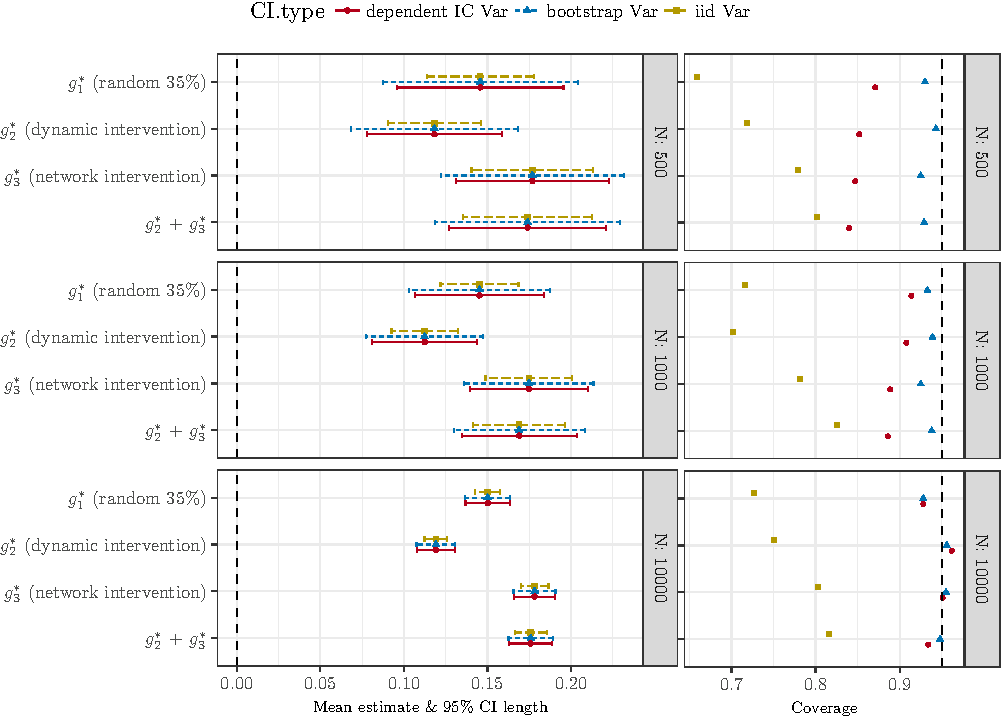
\includegraphics[width=\maxwidth]{TablesFigs/knitR-CIres_EY_prefattach-1} 

}

\caption[Mean 95\% CI length (left panel) and coverage (right panel) for the preferential attachment network, by sample size, interevention and CI type]{Mean 95\% CI length (left panel) and coverage (right panel) for the preferential attachment network, by sample size, interevention and CI type. Results shown for average expected outcomes only.}\label{fig:CIres.EY.prefattach}
\end{figure}


\end{knitrout}

\begin{knitrout}\footnotesize
\definecolor{shadecolor}{rgb}{0.969, 0.969, 0.969}\color{fgcolor}\begin{figure}

{\centering 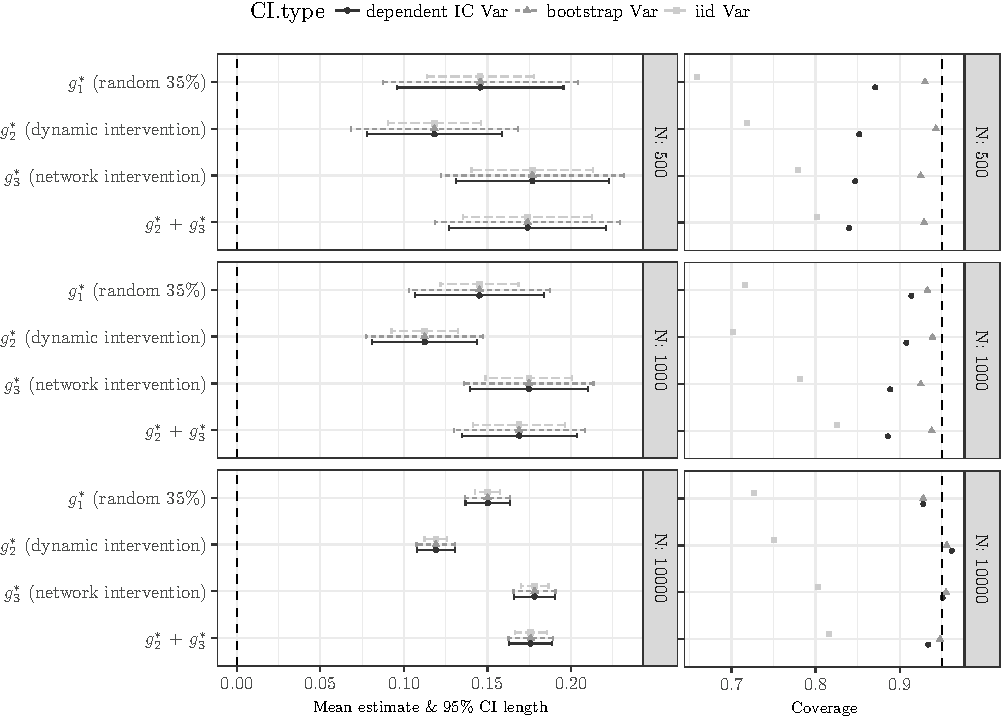
\includegraphics[width=\maxwidth]{TablesFigs/knitR-CIres_EY_prefattach_bw-1} 

}

\caption[Mean 95\% CI length (left panel) and coverage (right panel) for the preferential attachment network, by sample size, interevention and CI type]{Mean 95\% CI length (left panel) and coverage (right panel) for the preferential attachment network, by sample size, interevention and CI type. Results shown for average expected outcomes only.}\label{fig:CIres.EY.prefattach.bw}
\end{figure}


\end{knitrout}

\begin{knitrout}\footnotesize
\definecolor{shadecolor}{rgb}{0.969, 0.969, 0.969}\color{fgcolor}\begin{figure}

{\centering 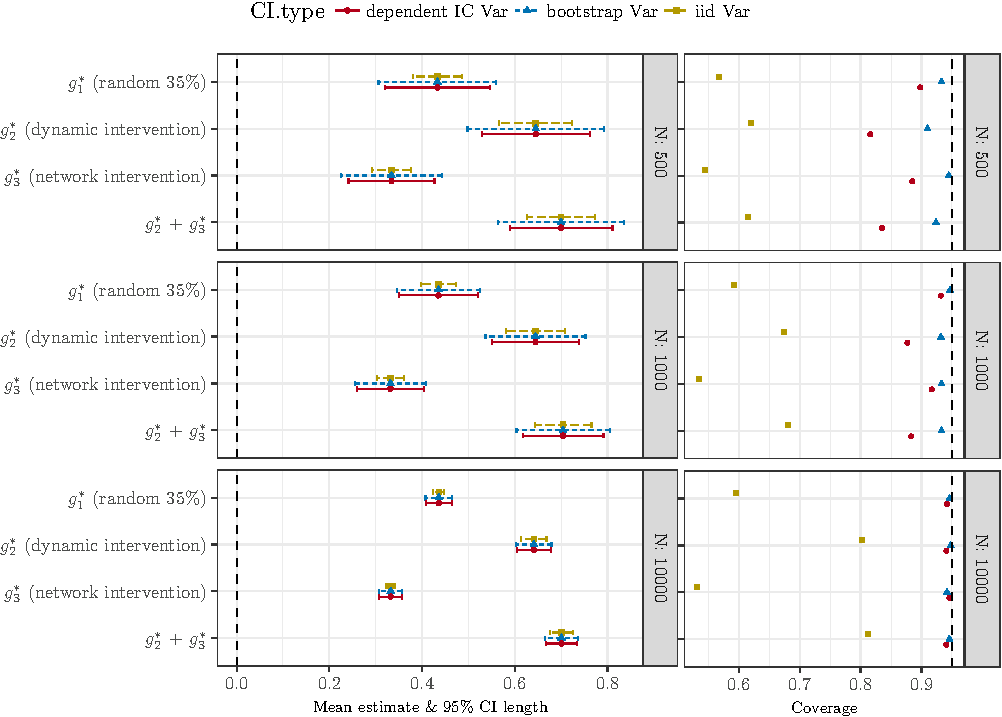
\includegraphics[width=\maxwidth]{TablesFigs/knitR-CIres_EY_smwld-1} 

}

\caption[Mean 95\% CI length (left panel) and coverage (right panel) for the small world network, by sample size, interevention and CI type]{Mean 95\% CI length (left panel) and coverage (right panel) for the small world network, by sample size, interevention and CI type. Results shown for average expected outcomes only.}\label{fig:CIres.EY.smwld}
\end{figure}


\end{knitrout}

\begin{knitrout}\footnotesize
\definecolor{shadecolor}{rgb}{0.969, 0.969, 0.969}\color{fgcolor}\begin{figure}

{\centering 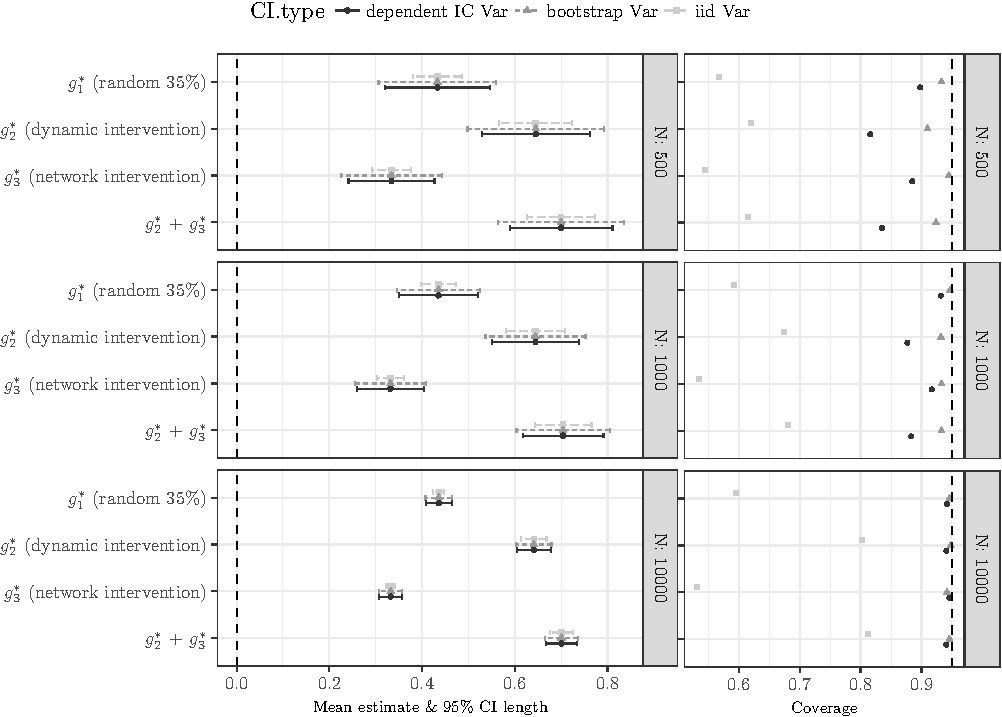
\includegraphics[width=\maxwidth]{TablesFigs/knitR-CIres_EY_smwld_bw-1} 

}

\caption[Mean 95\% CI length (left panel) and coverage (right panel) for the small world network, by sample size, interevention and CI type]{Mean 95\% CI length (left panel) and coverage (right panel) for the small world network, by sample size, interevention and CI type. Results shown for average expected outcomes only.}\label{fig:CIres.EY.smwld.bw}
\end{figure}


\end{knitrout}

\begin{knitrout}\footnotesize
\definecolor{shadecolor}{rgb}{0.969, 0.969, 0.969}\color{fgcolor}\begin{figure}

{\centering 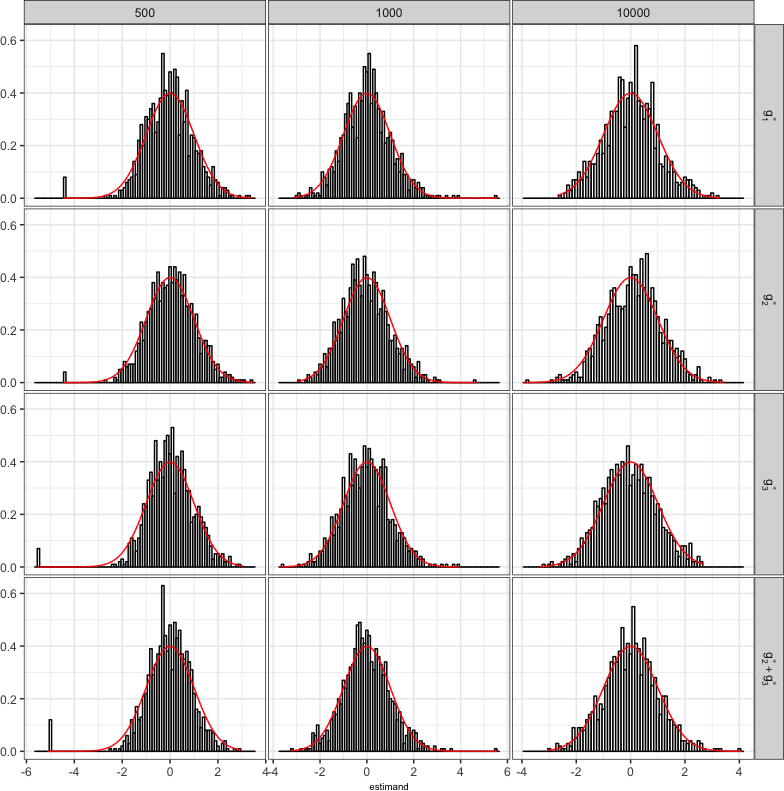
\includegraphics[width=\maxwidth]{TablesFigs/knitR-hist_TMLE_EY_prefattach-1} 

}

\caption[Distribution of the transformed TMLE (black) compared to the theoretical limiting distribution (red) by sample size (x-axis) and intervention type (y-axis)]{Distribution of the transformed TMLE (black) compared to the theoretical limiting distribution (red) by sample size (x-axis) and intervention type (y-axis). The estimates were centered at the truth and re-scaled by true SD. Results shown are for average expected outcomes in the preferential attachment network.}\label{fig:hist.TMLE.EY.prefattach}
\end{figure}


\end{knitrout}

\begin{knitrout}\footnotesize
\definecolor{shadecolor}{rgb}{0.969, 0.969, 0.969}\color{fgcolor}\begin{figure}

{\centering 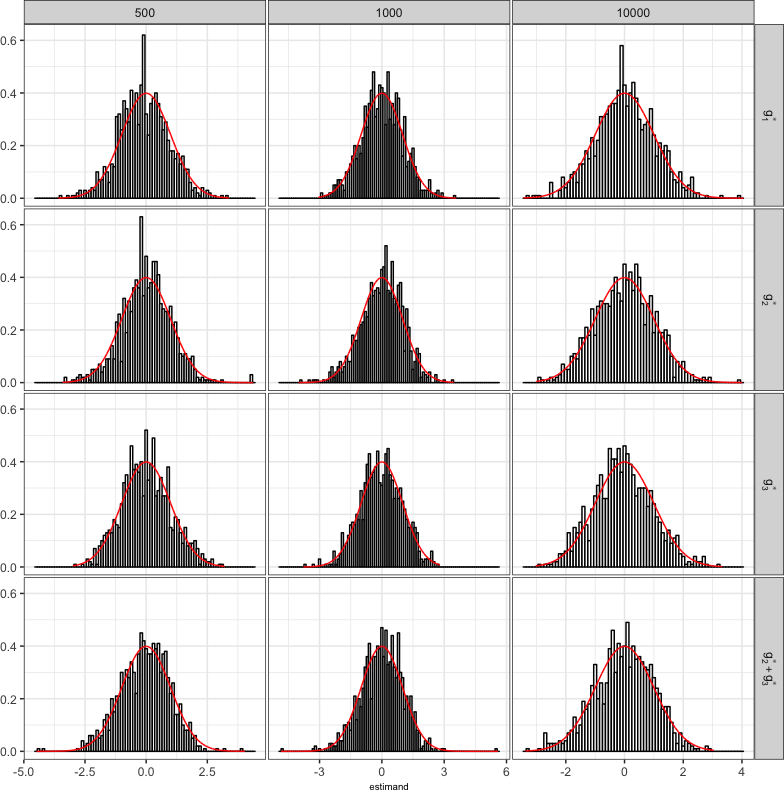
\includegraphics[width=\maxwidth]{TablesFigs/knitR-hist_TMLE_EY_smwld-1} 

}

\caption[Distribution of the transformed TMLE (black) compared to the theoretical limiting distribution (red) by sample size (x-axis) and intervention type (y-axis)]{Distribution of the transformed TMLE (black) compared to the theoretical limiting distribution (red) by sample size (x-axis) and intervention type (y-axis). The estimates were centered at the truth and re-scaled by true SD. Results shown are for average expected outcomes in the small world network.}\label{fig:hist.TMLE.EY.smwld}
\end{figure}


\end{knitrout}

% ------------------------------------------------------------------------------------------------------------
\newpage
\section{Supplementary results}
% ------------------------------------------------------------------------------------------------------------
\begin{knitrout}\footnotesize
\definecolor{shadecolor}{rgb}{0.969, 0.969, 0.969}\color{fgcolor}\begin{figure}

{\centering 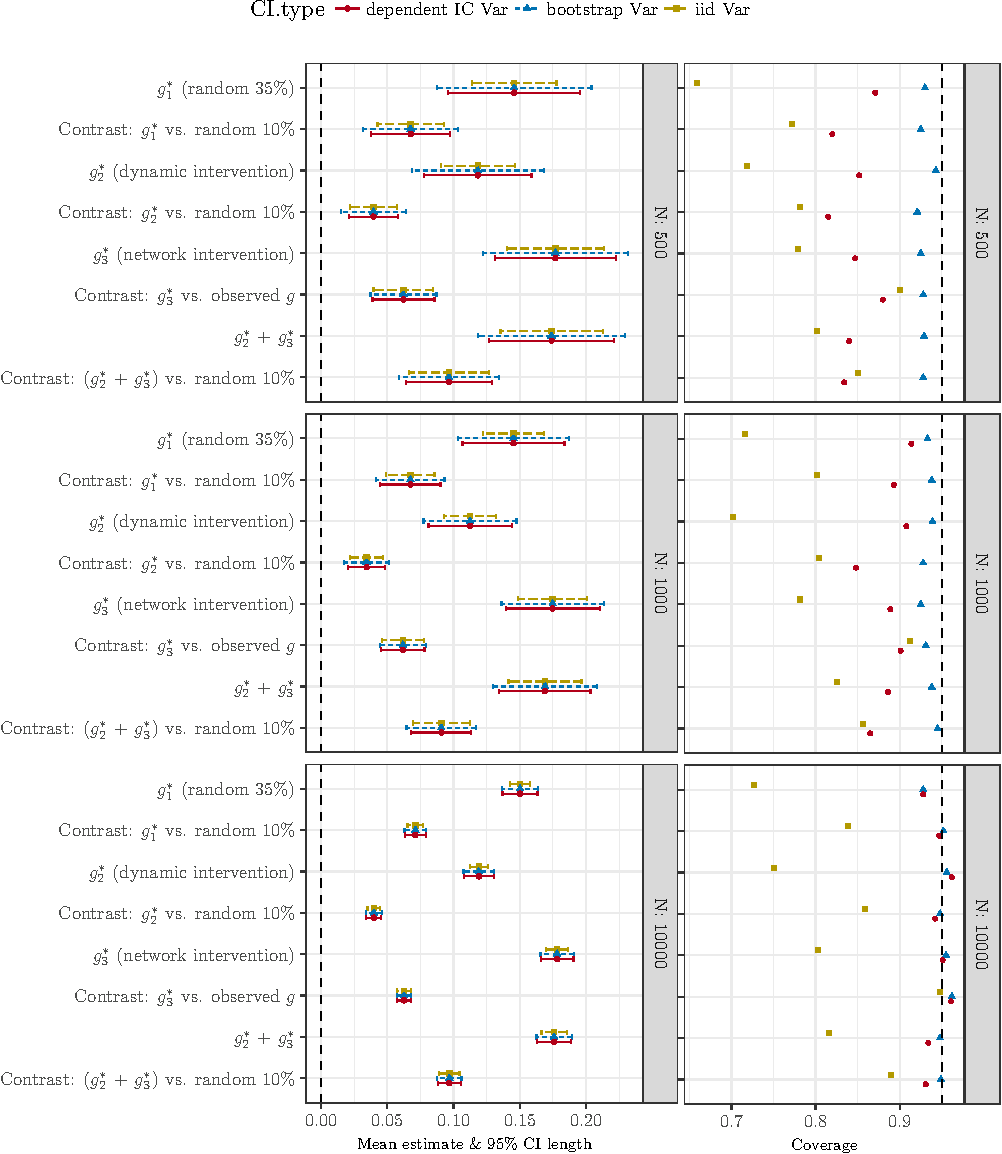
\includegraphics[width=\maxwidth]{TablesFigs/knitR-CIres_ALL_prefattach-1} 

}

\caption[Mean 95\% CI length (left panel) and coverage (right panel) for the preferential attachment network, by sample size, interevention and CI type]{Mean 95\% CI length (left panel) and coverage (right panel) for the preferential attachment network, by sample size, interevention and CI type. Results shown for all scenarios.}\label{fig:CIres.ALL.prefattach}
\end{figure}


\end{knitrout}

\begin{knitrout}\footnotesize
\definecolor{shadecolor}{rgb}{0.969, 0.969, 0.969}\color{fgcolor}\begin{figure}

{\centering 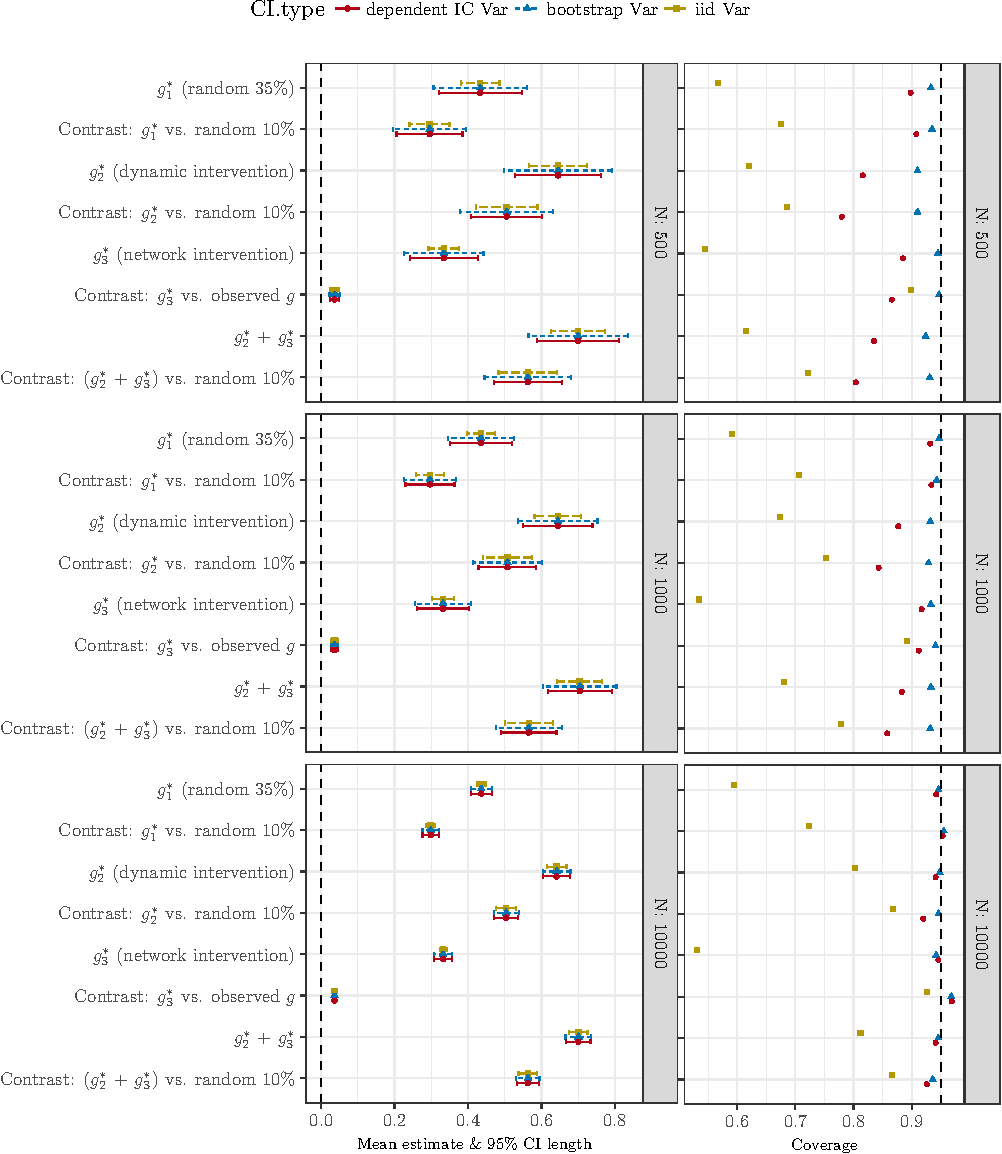
\includegraphics[width=\maxwidth]{TablesFigs/knitR-CIres_ALL_smwld-1} 

}

\caption[Mean 95\% CI length (left panel) and coverage (right panel) for the small world network, by sample size, interevention and CI type]{Mean 95\% CI length (left panel) and coverage (right panel) for the small world network, by sample size, interevention and CI type. Results shown for all scenarios.}\label{fig:CIres.ALL.smwld}
\end{figure}


\end{knitrout}

\begin{knitrout}\footnotesize
\definecolor{shadecolor}{rgb}{0.969, 0.969, 0.969}\color{fgcolor}\begin{figure}

{\centering 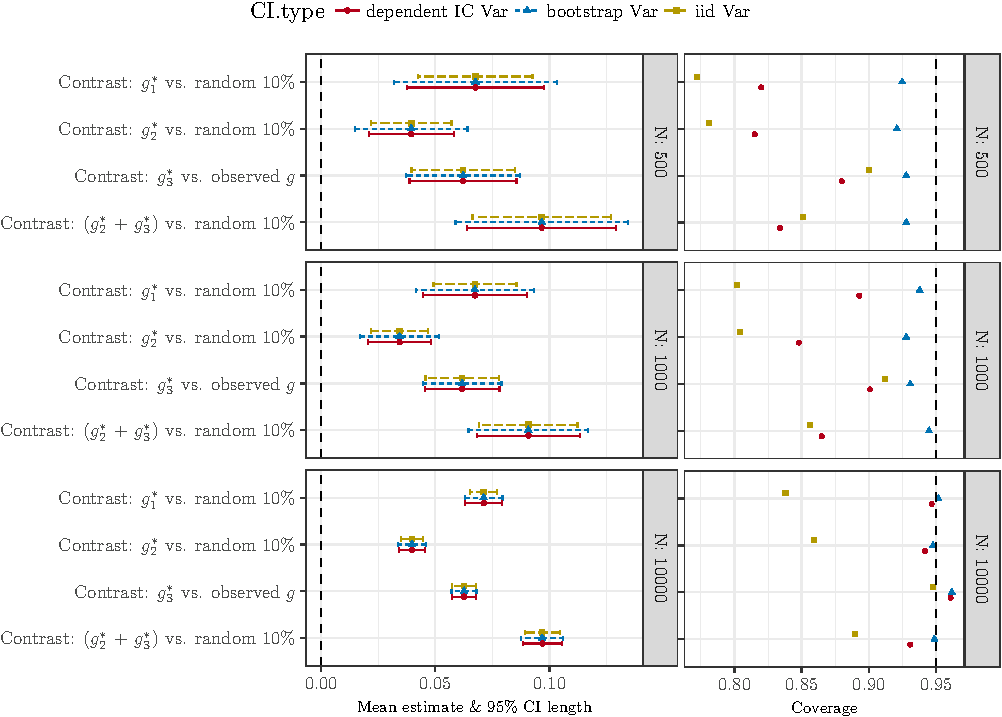
\includegraphics[width=\maxwidth]{TablesFigs/knitR-CIres_ATE_prefattach-1} 

}

\caption[Mean 95\% CI length (left panel) and coverage (right panel) for the preferential attachment network, by sample size, interevention and CI type]{Mean 95\% CI length (left panel) and coverage (right panel) for the preferential attachment network, by sample size, interevention and CI type. Results shown for contrasts only.}\label{fig:CIres.ATE.prefattach}
\end{figure}


\end{knitrout}

\begin{knitrout}\footnotesize
\definecolor{shadecolor}{rgb}{0.969, 0.969, 0.969}\color{fgcolor}\begin{figure}

{\centering 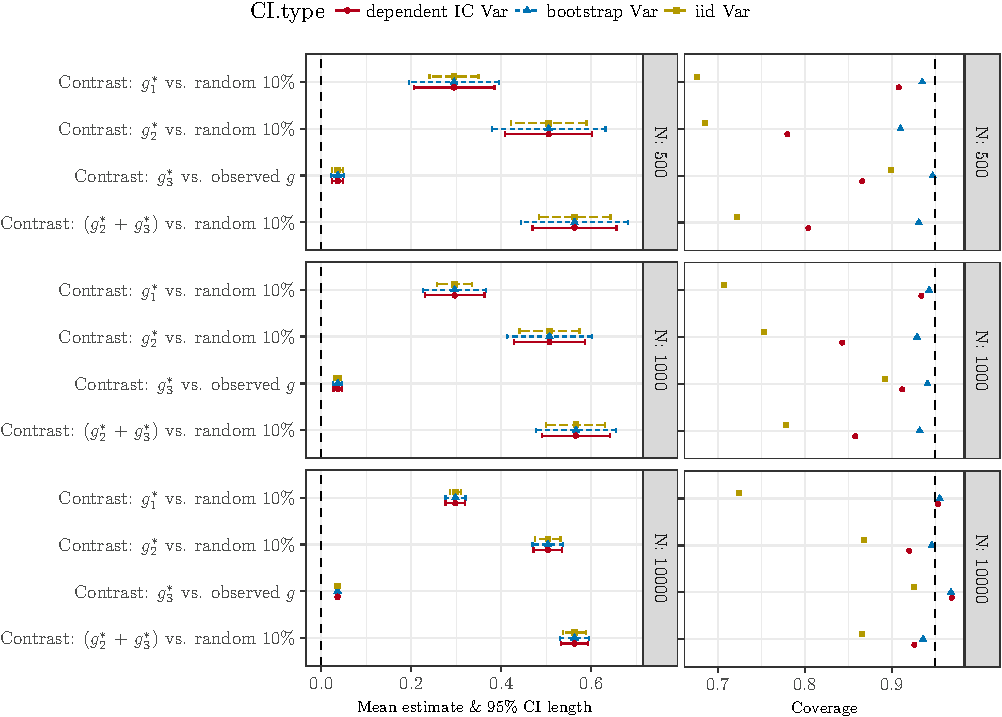
\includegraphics[width=\maxwidth]{TablesFigs/knitR-CIres_ATE_smwld-1} 

}

\caption[Mean 95\% CI length (left panel) and coverage (right panel) for the small world network, by sample size, interevention and CI type]{Mean 95\% CI length (left panel) and coverage (right panel) for the small world network, by sample size, interevention and CI type. Results shown for contrasts only.}\label{fig:CIres.ATE.smwld}
\end{figure}


\end{knitrout}

% ------------------------------------------------------------------------------------------------------------
% TMLE RESULTS (ATE)
% ------------------------------------------------------------------------------------------------------------
\begin{knitrout}\footnotesize
\definecolor{shadecolor}{rgb}{0.969, 0.969, 0.969}\color{fgcolor}\begin{figure}

{\centering 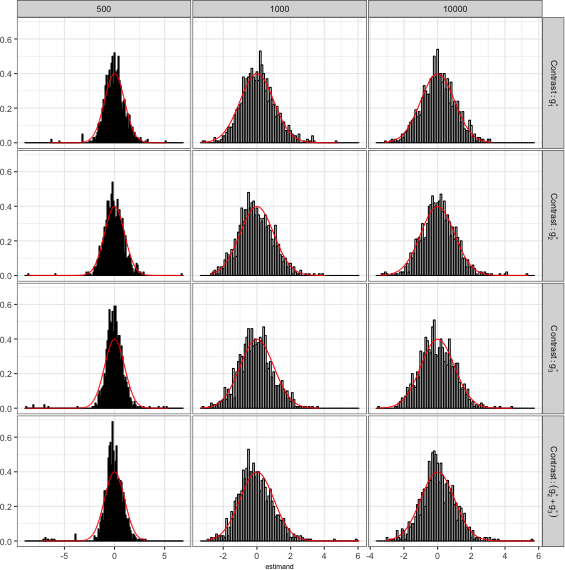
\includegraphics[width=\maxwidth]{TablesFigs/knitR-hist_TMLE_ATE_prefattach-1} 

}

\caption[Distribution of the transformed TMLE (black) compared to the theoretical limiting distribution (red) by sample size (x-axis) and intervention type (y-axis)]{Distribution of the transformed TMLE (black) compared to the theoretical limiting distribution (red) by sample size (x-axis) and intervention type (y-axis). The estimates were centered at the truth and re-scaled by true SD. Results shown are for contrasts in preferential attachment network.}\label{fig:hist.TMLE.ATE.prefattach}
\end{figure}


\end{knitrout}
\begin{knitrout}\footnotesize
\definecolor{shadecolor}{rgb}{0.969, 0.969, 0.969}\color{fgcolor}\begin{figure}

{\centering 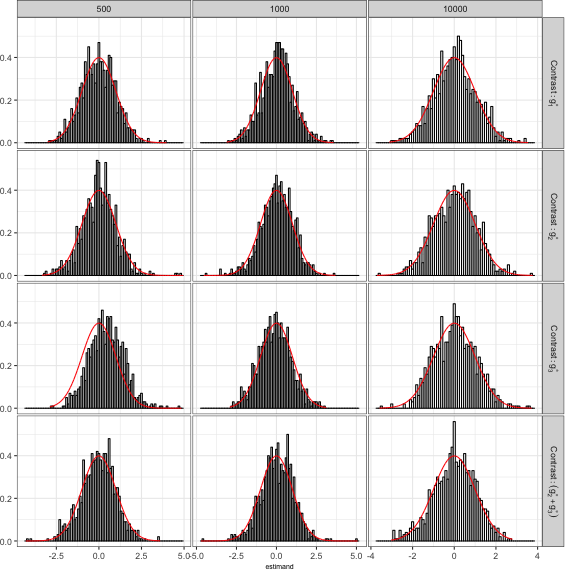
\includegraphics[width=\maxwidth]{TablesFigs/knitR-hist_TMLE_ATE_smwld-1} 

}

\caption[Distribution of the transformed TMLE (black) compared to the theoretical limiting distribution (red) by sample size (x-axis) and intervention type (y-axis)]{Distribution of the transformed TMLE (black) compared to the theoretical limiting distribution (red) by sample size (x-axis) and intervention type (y-axis). The estimates were centered at the truth and re-scaled by true SD. Results shown are for contrasts in small world network.}\label{fig:hist.TMLE.ATE.smwld}
\end{figure}


\end{knitrout}

% ------------------------------------------------------------------------------------------------------------
% IPTW RESULTS (EY and ATE)
% ------------------------------------------------------------------------------------------------------------
\begin{knitrout}\footnotesize
\definecolor{shadecolor}{rgb}{0.969, 0.969, 0.969}\color{fgcolor}\begin{figure}

{\centering 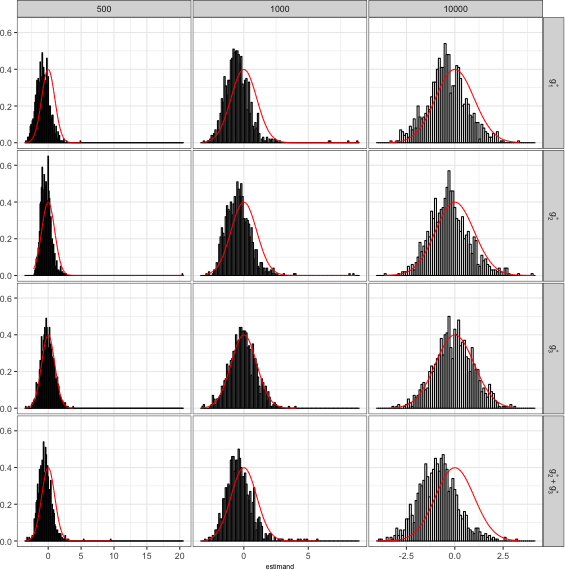
\includegraphics[width=\maxwidth]{TablesFigs/knitR-hist_IPTW_EY_prefattach-1} 

}

\caption[Distribution of the transformed IPTW (black) compared to the theoretical limiting distribution (red) by sample size (x-axis) and intervention type (y-axis)]{Distribution of the transformed IPTW (black) compared to the theoretical limiting distribution (red) by sample size (x-axis) and intervention type (y-axis). The estimates were centered at the truth and re-scaled by true SD. Results shown are for average expected outcomes in the preferential attachment network.}\label{fig:hist.IPTW.EY.prefattach}
\end{figure}


\end{knitrout}

\begin{knitrout}\footnotesize
\definecolor{shadecolor}{rgb}{0.969, 0.969, 0.969}\color{fgcolor}\begin{figure}

{\centering 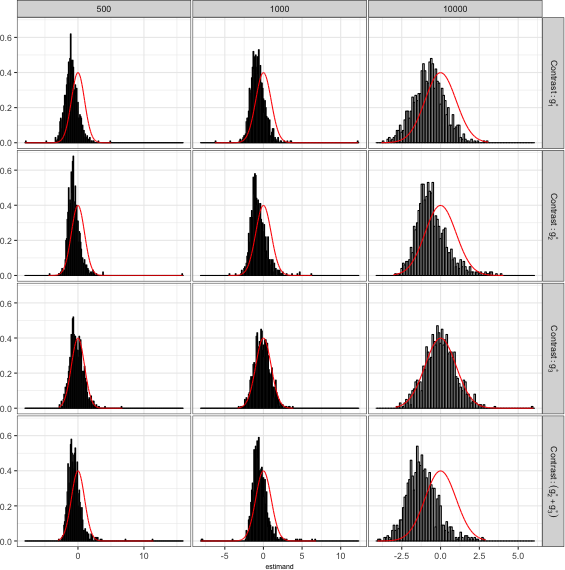
\includegraphics[width=\maxwidth]{TablesFigs/knitR-hist_IPTW_ATE_prefattach-1} 

}

\caption[Distribution of the transformed IPTW (black) compared to the theoretical limiting distribution (red) by sample size (x-axis) and intervention type (y-axis)]{Distribution of the transformed IPTW (black) compared to the theoretical limiting distribution (red) by sample size (x-axis) and intervention type (y-axis). The estimates were centered at the truth and re-scaled by true SD. Results shown are for contrasts in the preferential attachment network.}\label{fig:hist.IPTW.ATE.prefattach}
\end{figure}


\end{knitrout}

\begin{knitrout}\footnotesize
\definecolor{shadecolor}{rgb}{0.969, 0.969, 0.969}\color{fgcolor}\begin{figure}

{\centering 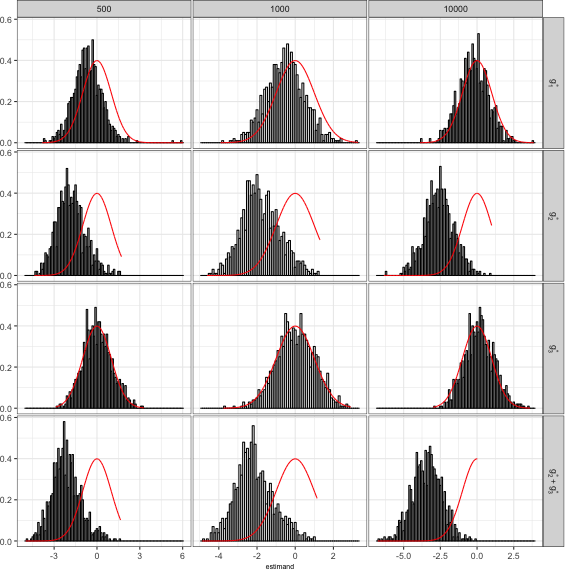
\includegraphics[width=\maxwidth]{TablesFigs/knitR-hist_IPTW_EY_smwld-1} 

}

\caption[Distribution of the transformed IPTW (black) compared to the theoretical limiting distribution (red) by sample size (x-axis) and intervention type (y-axis)]{Distribution of the transformed IPTW (black) compared to the theoretical limiting distribution (red) by sample size (x-axis) and intervention type (y-axis). The estimates were centered at the truth and re-scaled by true SD. Results shown are for average expected outcomes in the small world network.}\label{fig:hist.IPTW.EY.smwld}
\end{figure}


\end{knitrout}

\begin{knitrout}\footnotesize
\definecolor{shadecolor}{rgb}{0.969, 0.969, 0.969}\color{fgcolor}\begin{figure}

{\centering 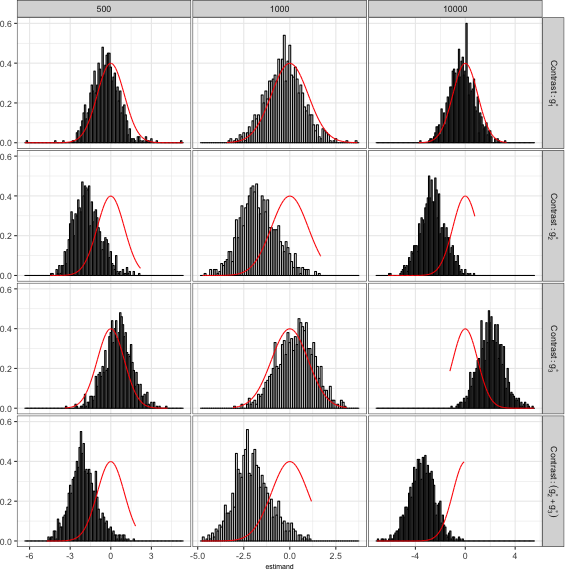
\includegraphics[width=\maxwidth]{TablesFigs/knitR-hist_IPTW_ATE_smwld-1} 

}

\caption[Distribution of the transformed IPTW (black) compared to the theoretical limiting distribution (red) by sample size (x-axis) and intervention type (y-axis)]{Distribution of the transformed IPTW (black) compared to the theoretical limiting distribution (red) by sample size (x-axis) and intervention type (y-axis). The estimates were centered at the truth and re-scaled by true SD. Results shown are for contrasts in the small world network.}\label{fig:hist.IPTW.ATE.smwld}
\end{figure}


\end{knitrout}

\end{document}

